\begin{frame}{Ausblick}
    \begin{columns}[T] % T aligns the tops of the columns
        \begin{column}{0.3\textwidth}
            \vspace*{0.5cm}
            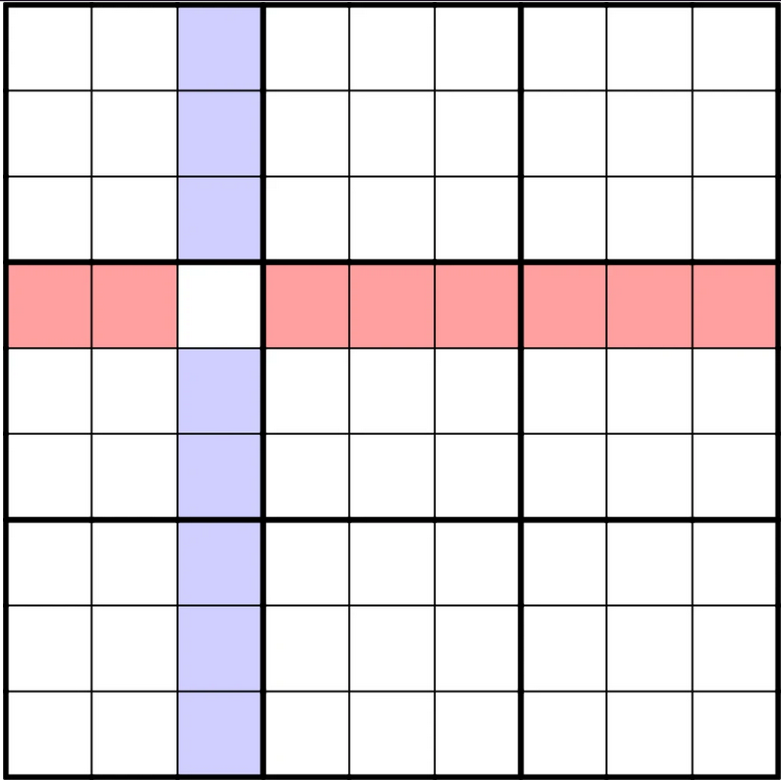
\includegraphics[width=\textwidth]{Pictures/H3.png} \\
            \vspace*{0.5cm}
            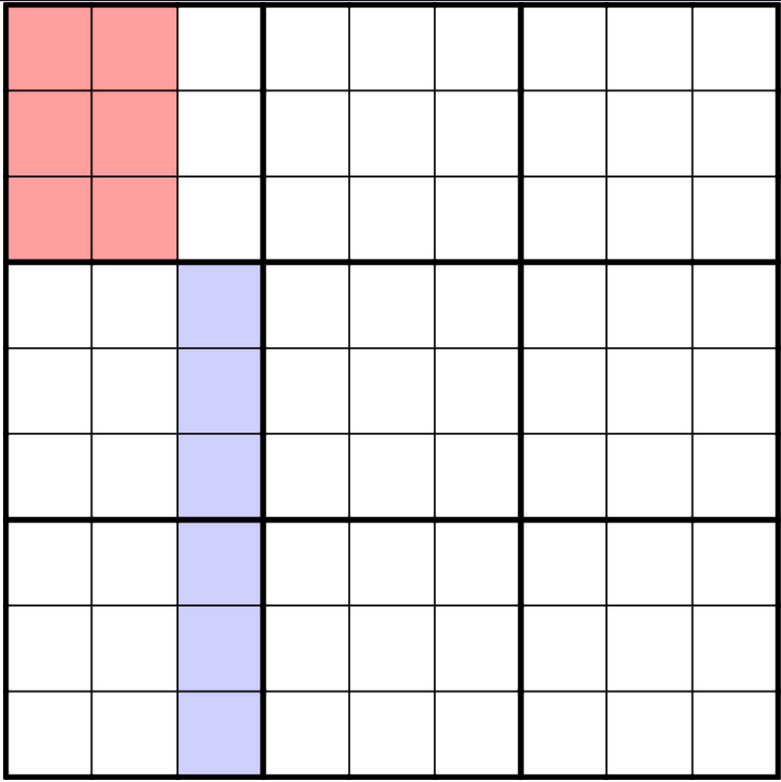
\includegraphics[width=\textwidth]{Pictures/H5.png}
        \end{column}
        \begin{column}{0.3\textwidth}
            \vspace*{0.5cm}
            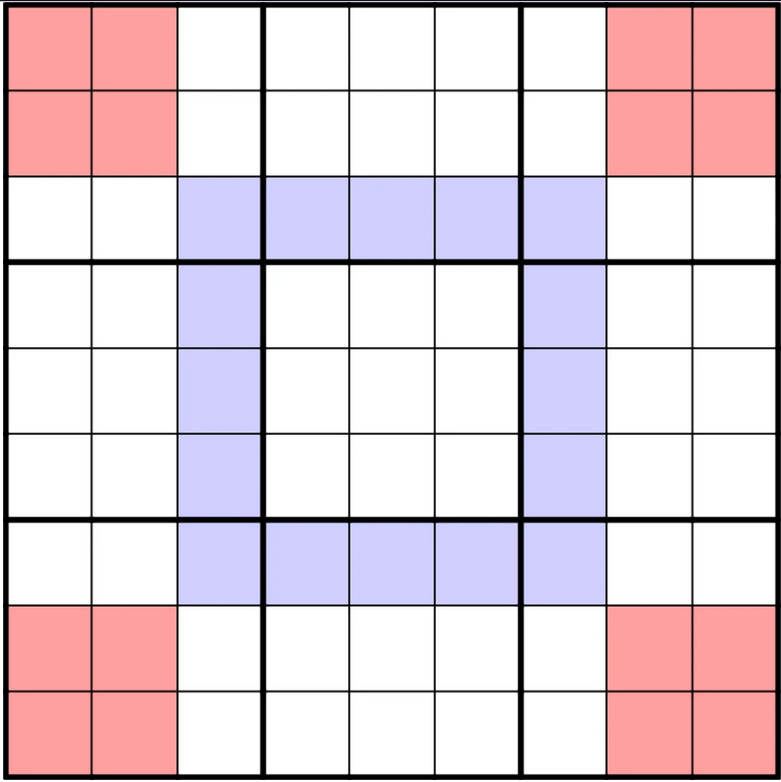
\includegraphics[width=\textwidth]{Pictures/H1.png} \\
            \vspace*{0.5cm}
            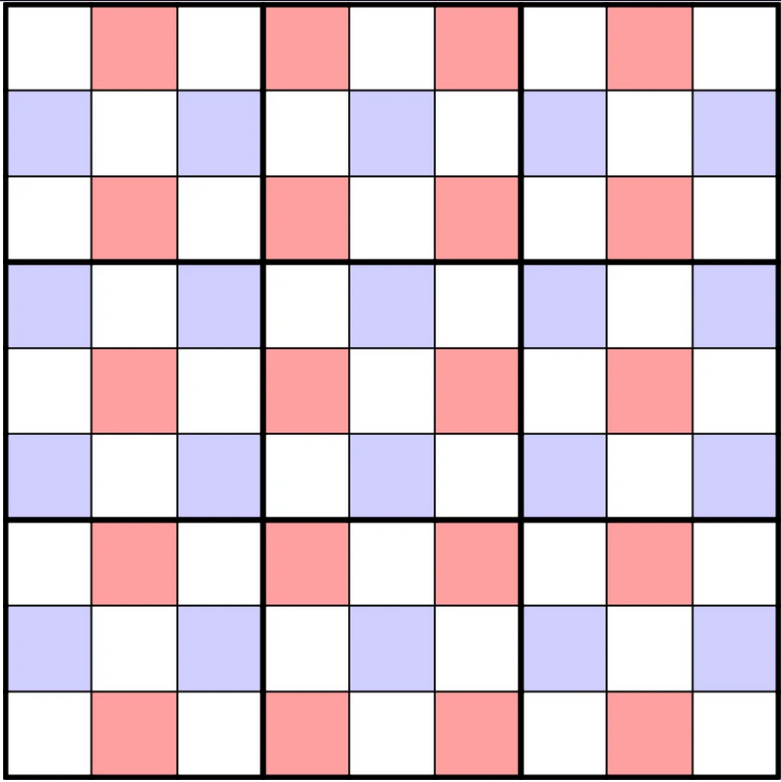
\includegraphics[width=\textwidth]{Pictures/H4.png}
            \cite{SET}
        \end{column}
        \begin{column}{0.35\textwidth}
            \vspace*{0.5cm}
            \begin{itemize}
                \item Anwenden von Set AEquivalenz Theorie (z.B. in Fitnessbewertung oder Mutation)
                \item mehr Exploration durch andere Selektionsverfahren
                \item Anpassung an andere Sudokuarten
            \end{itemize}
        \end{column}
    \end{columns}
    \note[item]{Anwenden von Set Aequivalenz Theorie (z.B. in Fitnessbewertung)}
    \note[item]{eventuell flexiblerer Selektionsdruck (um zu Beginn mehr Exploration zu haben)}
    \note[item]{Anpassung an andere Sudokuarten, z.B. Freiform Sudoku oder groessere Arten}
    \note[item]{GUI-Erklaeren}
\end{frame}